\setAuthor{Jaan Kalda}
\setRound{lahtine}
\setYear{2020}
\setNumber{G 10}
\setDifficulty{10}
\setTopic{TODO}

\prob{Koonus}
Vabalt painduva venimatu niidi otstes on kuulid massidega $m$ ja $2m$, vt joonist. Kuul massiga $2m$ lebab koonilisel pinnal, mis moodustab horisondiga nurga $\alpha=30^\circ$, raskuskiirendus $g$ on vertikaalselt alla suunatud. Alghetkel on niit pingul ja koonusel lebava kuuli kiirusvektor mooduliga $v_0$ lebab koonuse pinna tasandis moodustades nurga $\beta$ niidiga (st kuuli ja koonuse tippu ühendava sihiga). Teine kuul liigub vertikaalselt niidi pinge ja raskusjõu koosmõjul, algkiirusega $v_0\cos\beta$. Kõiki hõõrdejõude võib ignoreerida.\\
	\osa Kui pika aja pärast  jõuab teine kuul oma teekonna madalaimasse punkti eeldusel, et esimene kuul püsib koonilisel pinnal?\\
	\osa Milline võrratus peab olema rahuldatud, et eelmises punktis tehtud eeldus kehtiks, st et kuulike ei kerkiks kooniliselt pinnalt õhku?
	
	\begin{center}
		\vspace{-13pt}
		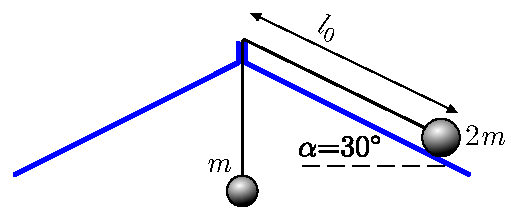
\includegraphics[width=0.55\linewidth]{2020-lahg-10-yl.pdf}
	\end{center}


\hint

\solu
\osa Vaatleme koonuse pinna tasandis toimivaid jõude. Nööri pinge tasakaalustab alati raskusjõu pinnasihilise komponendi, seega pinnasihilised jõud puuduvad, mistõttu liigub kuulike koonuse pinnalaotusel mööda sirgjoont. Seetõttu on teepikkus pinnalaotusel algasendist kuni suurima lähenemiseni tipule $L=l_0\cos\beta$ ning seega otsitav aeg $t=L/v_0=l_0\cos\beta/v_0$. 

\osa Ilmselt on õhku hüppamise mõttes kõige ohtlikum koonilist pinda mööda liikuva kuulikese trajektoori kõrgeim punkt, mille kaugus tipust on $l_0\sin\beta$. Kuivõrd tegemist on kõrgeima punktiga, siis on trajektoori puutujatasand seal horisontaalne ning trajektoori kõverusraadius võrdne antud punkti kaugusega koonuse teljest: $R=l_0\sin\beta\cos\alpha$. Seega on kuulikese kesktõmbekiirendus $a=v_0^2/R$ suunatud horisontaalselt telje suunas. Piirjuhul on selle kiirenduse pinnanormaali sihiline komponent $v_0^2\sin\alpha/R$ võrdne vastava raskuskiirenduse komponendiga $g\cos\alpha$. Seega saame tingimuseks $v_0^2\tan\alpha\le gl_0\sin\beta\cos\alpha$, st $$v_0^2\le \frac{3}{2}gl_0\sin\beta.$$
\probend